\documentclass[10pt]{beamer}

\usepackage{appendixnumberbeamer}
\usepackage{booktabs}
\usepackage[scale=2]{ccicons}
\usepackage{pgfplots}
\usepackage{graphics}
\usepackage{braket}

\usepgfplotslibrary{dateplot}
\pdfstringdefDisableCommands{\def\translate#1{#1}}
\geometry{paperwidth=140mm, paperheight=105mm}
\usetheme{metropolis}
\bibliographystyle{abbrv}
\setbeamertemplate{frame footer}{ME738 - Special Topics in Materials}

\renewcommand{\footnotesize}{\fontsize{7pt}{8pt}\selectfont}

\title{Chip Scale Atomic Clocks Sources}
\subtitle{Applications}
\date{March 27, 2024}
\author{Tommaso Bocchietti}
\institute{University of Waterloo}
\titlegraphic{\hfill
\includegraphics[height=1.5cm]{pdf/UniversityOfWaterloo_logo_horiz_pms.pdf}}

\begin{document}

\maketitle

\begin{frame}{Agenda}
    \setbeamertemplate{section in toc}[sections numbered]
    \tableofcontents[hideallsubsections]
\end{frame}

\begin{frame}{Recap from "Technology comparison"}

    The \textit{absolute best} CSACs doesn't exist.

    \vspace{10pt}

    In general, performance of the clock are proportional to its SWaP (Size Weight and Power) and cost.

    \vspace{10pt}

    The choice of the clock depends on the application requirements.

\end{frame}

\section{Global Navigation Satellite Systems (GNSS)}

\begin{frame}{Trilateration in GNSS networks}

    System of equations involved in trilateration \textbf{($\delta t$ is the receiver clock delay)}:

    \begin{equation*}
        \Delta d_i = c \cdot (\Delta t_i + \delta t) = \sqrt{(x_r - x_i)^2 + (y_r - y_i)^2 + (z_r - z_i)^2}, \quad i = 1, 2, 3, 4
    \end{equation*}

    \begin{columns}[c, onlytextwidth]

        \begin{column}{0.6\textwidth}

            \begin{equation*}
                \underbrace{x_r, y_r, z_r, \delta t}_\text{4 Unknowns requires 4 satellites}
            \end{equation*}

            \vspace{10pt}

            \textbf{Final position strongly depends on $\delta t$.}

        \end{column}

        \begin{column}{0.4\textwidth}

            \begin{figure}[H]
                \centering
                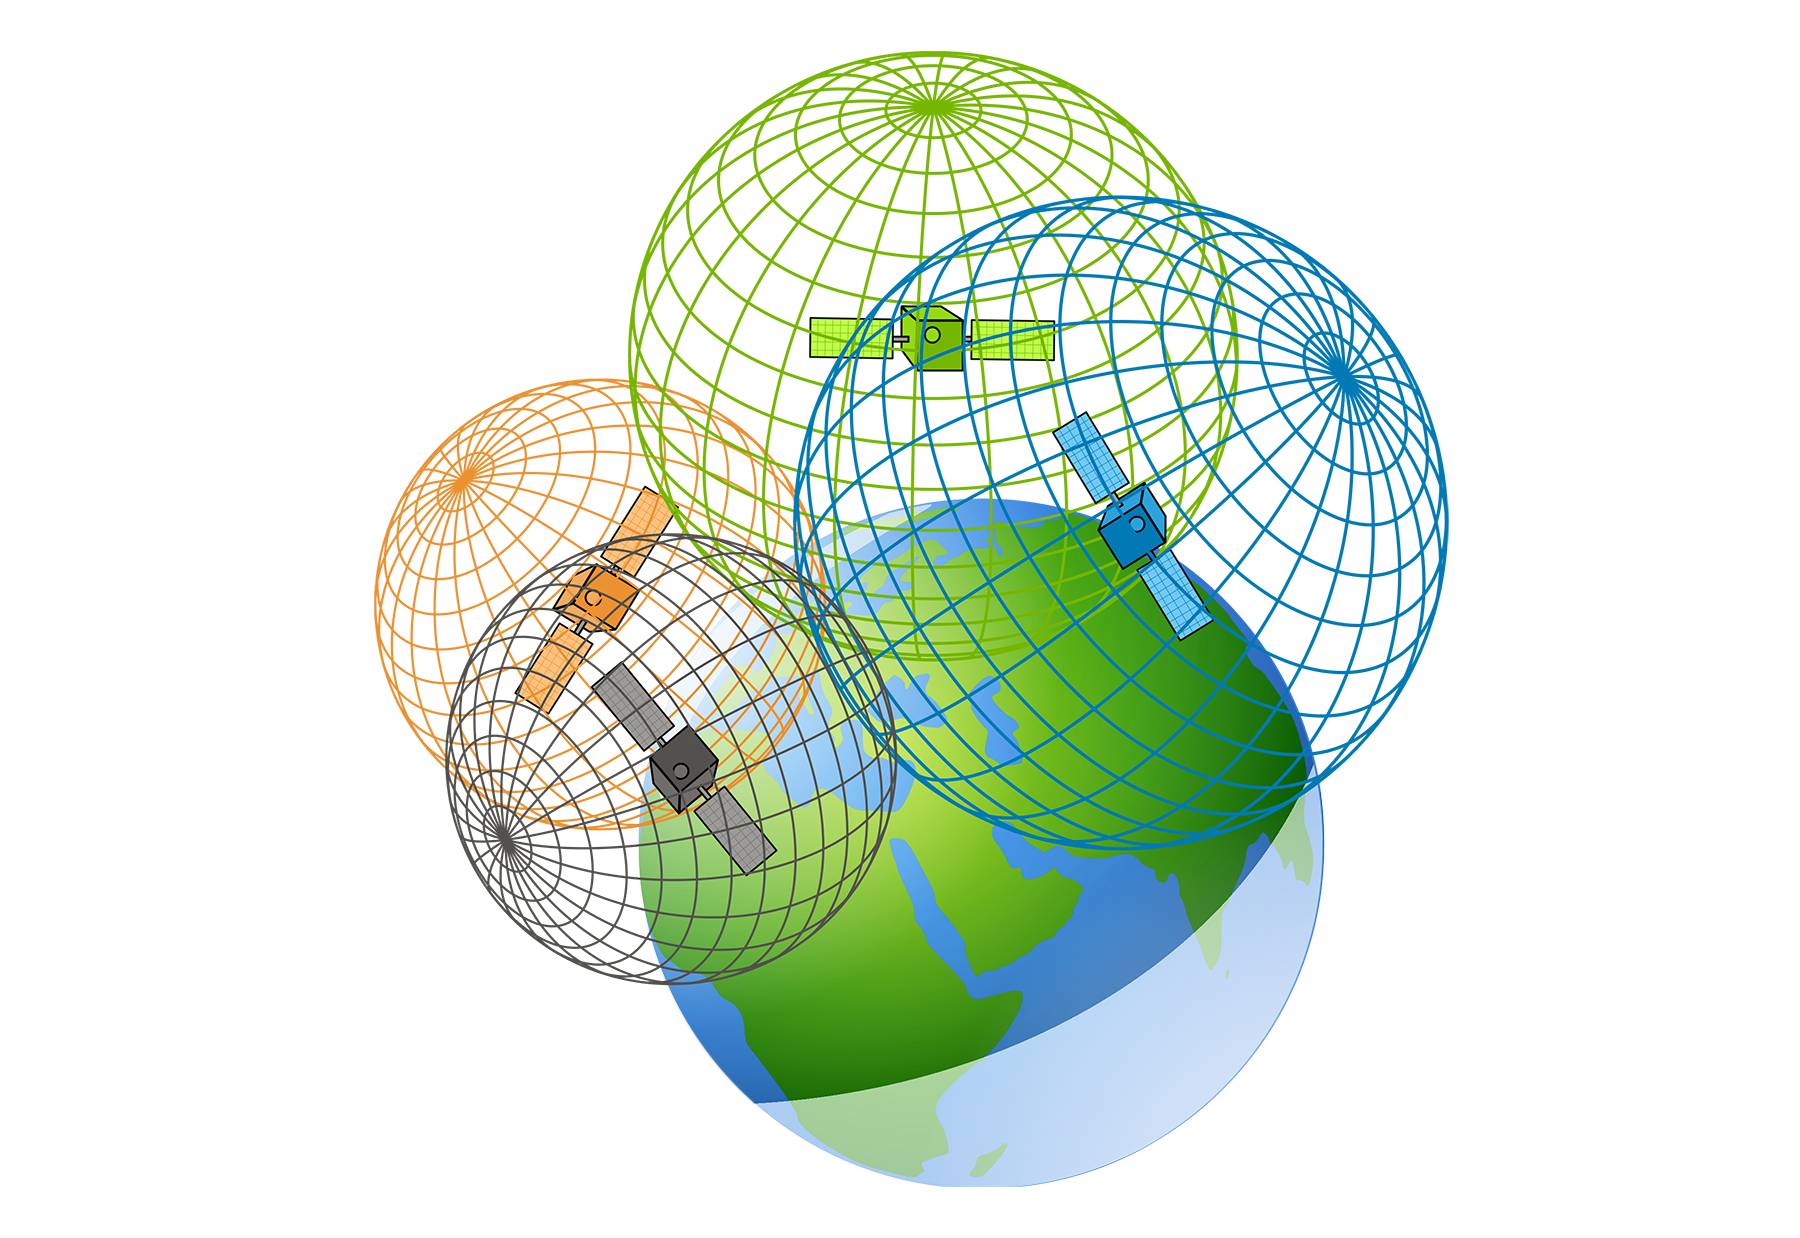
\includegraphics[width=\textwidth]{img/GPS-Trilateration.png}
                % \caption{GPS trilateration}
            \end{figure}

        \end{column}

    \end{columns}

    \footnotetext{In the equation above, $c$ is the speed of light which is approximately $3 \times 10^8$ m/s.}

\end{frame}



% \begin{frame}{Role of CSAC}

%     Better holdover capabilities $\rightarrow$ eliminate the need for the 4\textsuperscript{th} satellite after the first clock calibration.

%     More accurate timing $\rightarrow$ more precise trilateration and indeed a more accurate position.

%     \vspace{10pt}

%     \begin{columns}[c, onlytextwidth]

%         \begin{column}{0.5\textwidth}

%             % TODO: change image, take the one from Travagning p.68
%             \begin{figure}
%                 \centering
%                 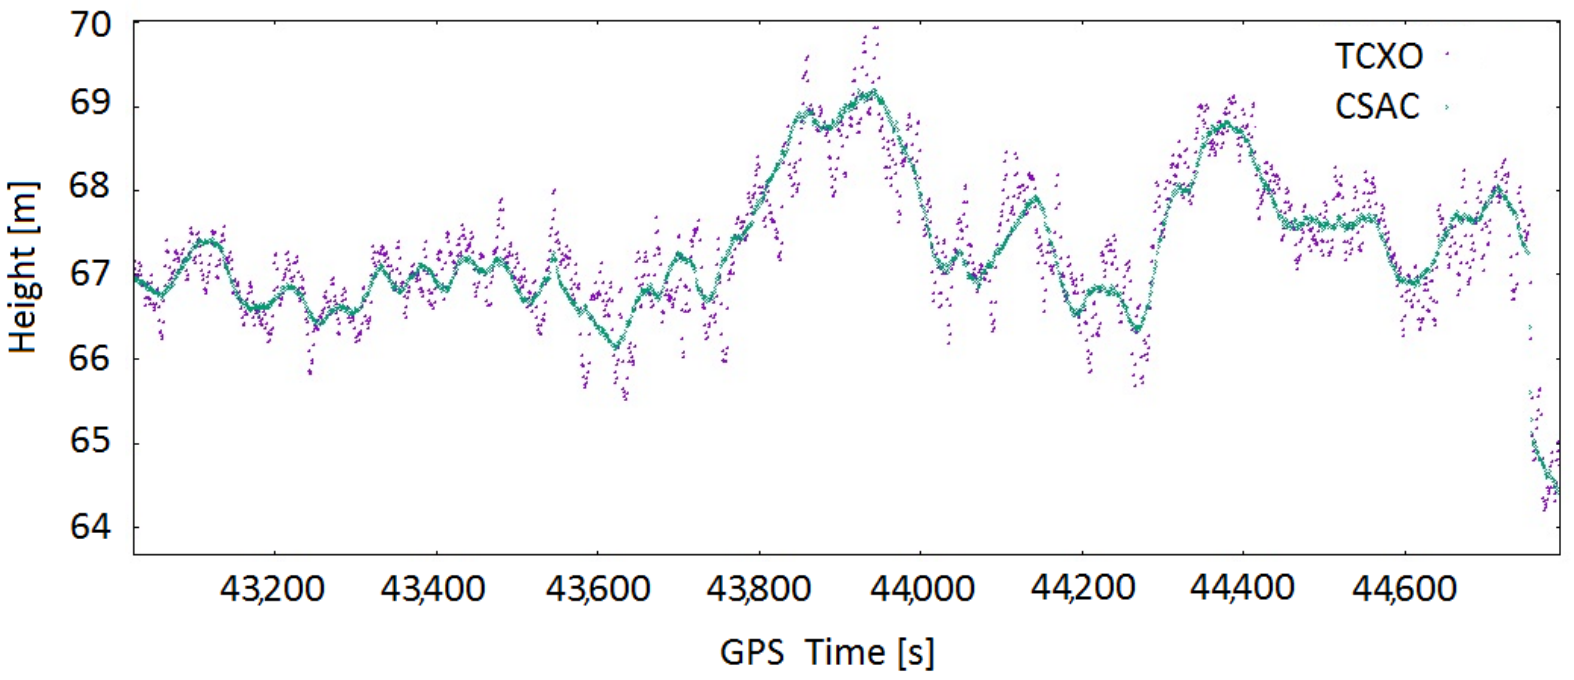
\includegraphics[width=\textwidth]{img/GNSS-height.png}
%                 \caption{
%                     \textcolor[HTML]{663B7A}{TCXO},
%                     \textcolor[HTML]{64857B}{CSAC}
%                 }
%             \end{figure}

%         \end{column}

%         \hfill

%         \begin{column}{0.45\textwidth}

%             \begin{table}
%                 \centering
%                 \resizebox{\textwidth}{!}{
%                     \begin{tabular}{l|cc}
%                         ~    & \textbf{Static} & \textbf{Dynamic} \\
%                         ~    & (cm)            & (cm)             \\
%                         \hline
%                         TCXO & 50.0            & 55.0             \\
%                         CSAC & 25.5            & 24.3             \\
%                         \hline
%                     \end{tabular}
%                 }
%                 \caption{Height error standard deviation in static and dynamic conditions.}
%             \end{table}

%         \end{column}

%     \end{columns}

% \end{frame}



\begin{frame}{Role of CSAC}

    \begin{columns}[c, onlytextwidth]

        \begin{column}{0.55\textwidth}

            Better holdover capabilities $\rightarrow$ eliminate the need for the 4\textsuperscript{th} satellite after the first clock calibration.

            \vspace{10pt}

            More accurate timing $\rightarrow$ more precise trilateration and indeed a more accurate position.

        \end{column}

        \hfill

        \begin{column}{0.40\textwidth}

            \begin{figure}
                \centering
                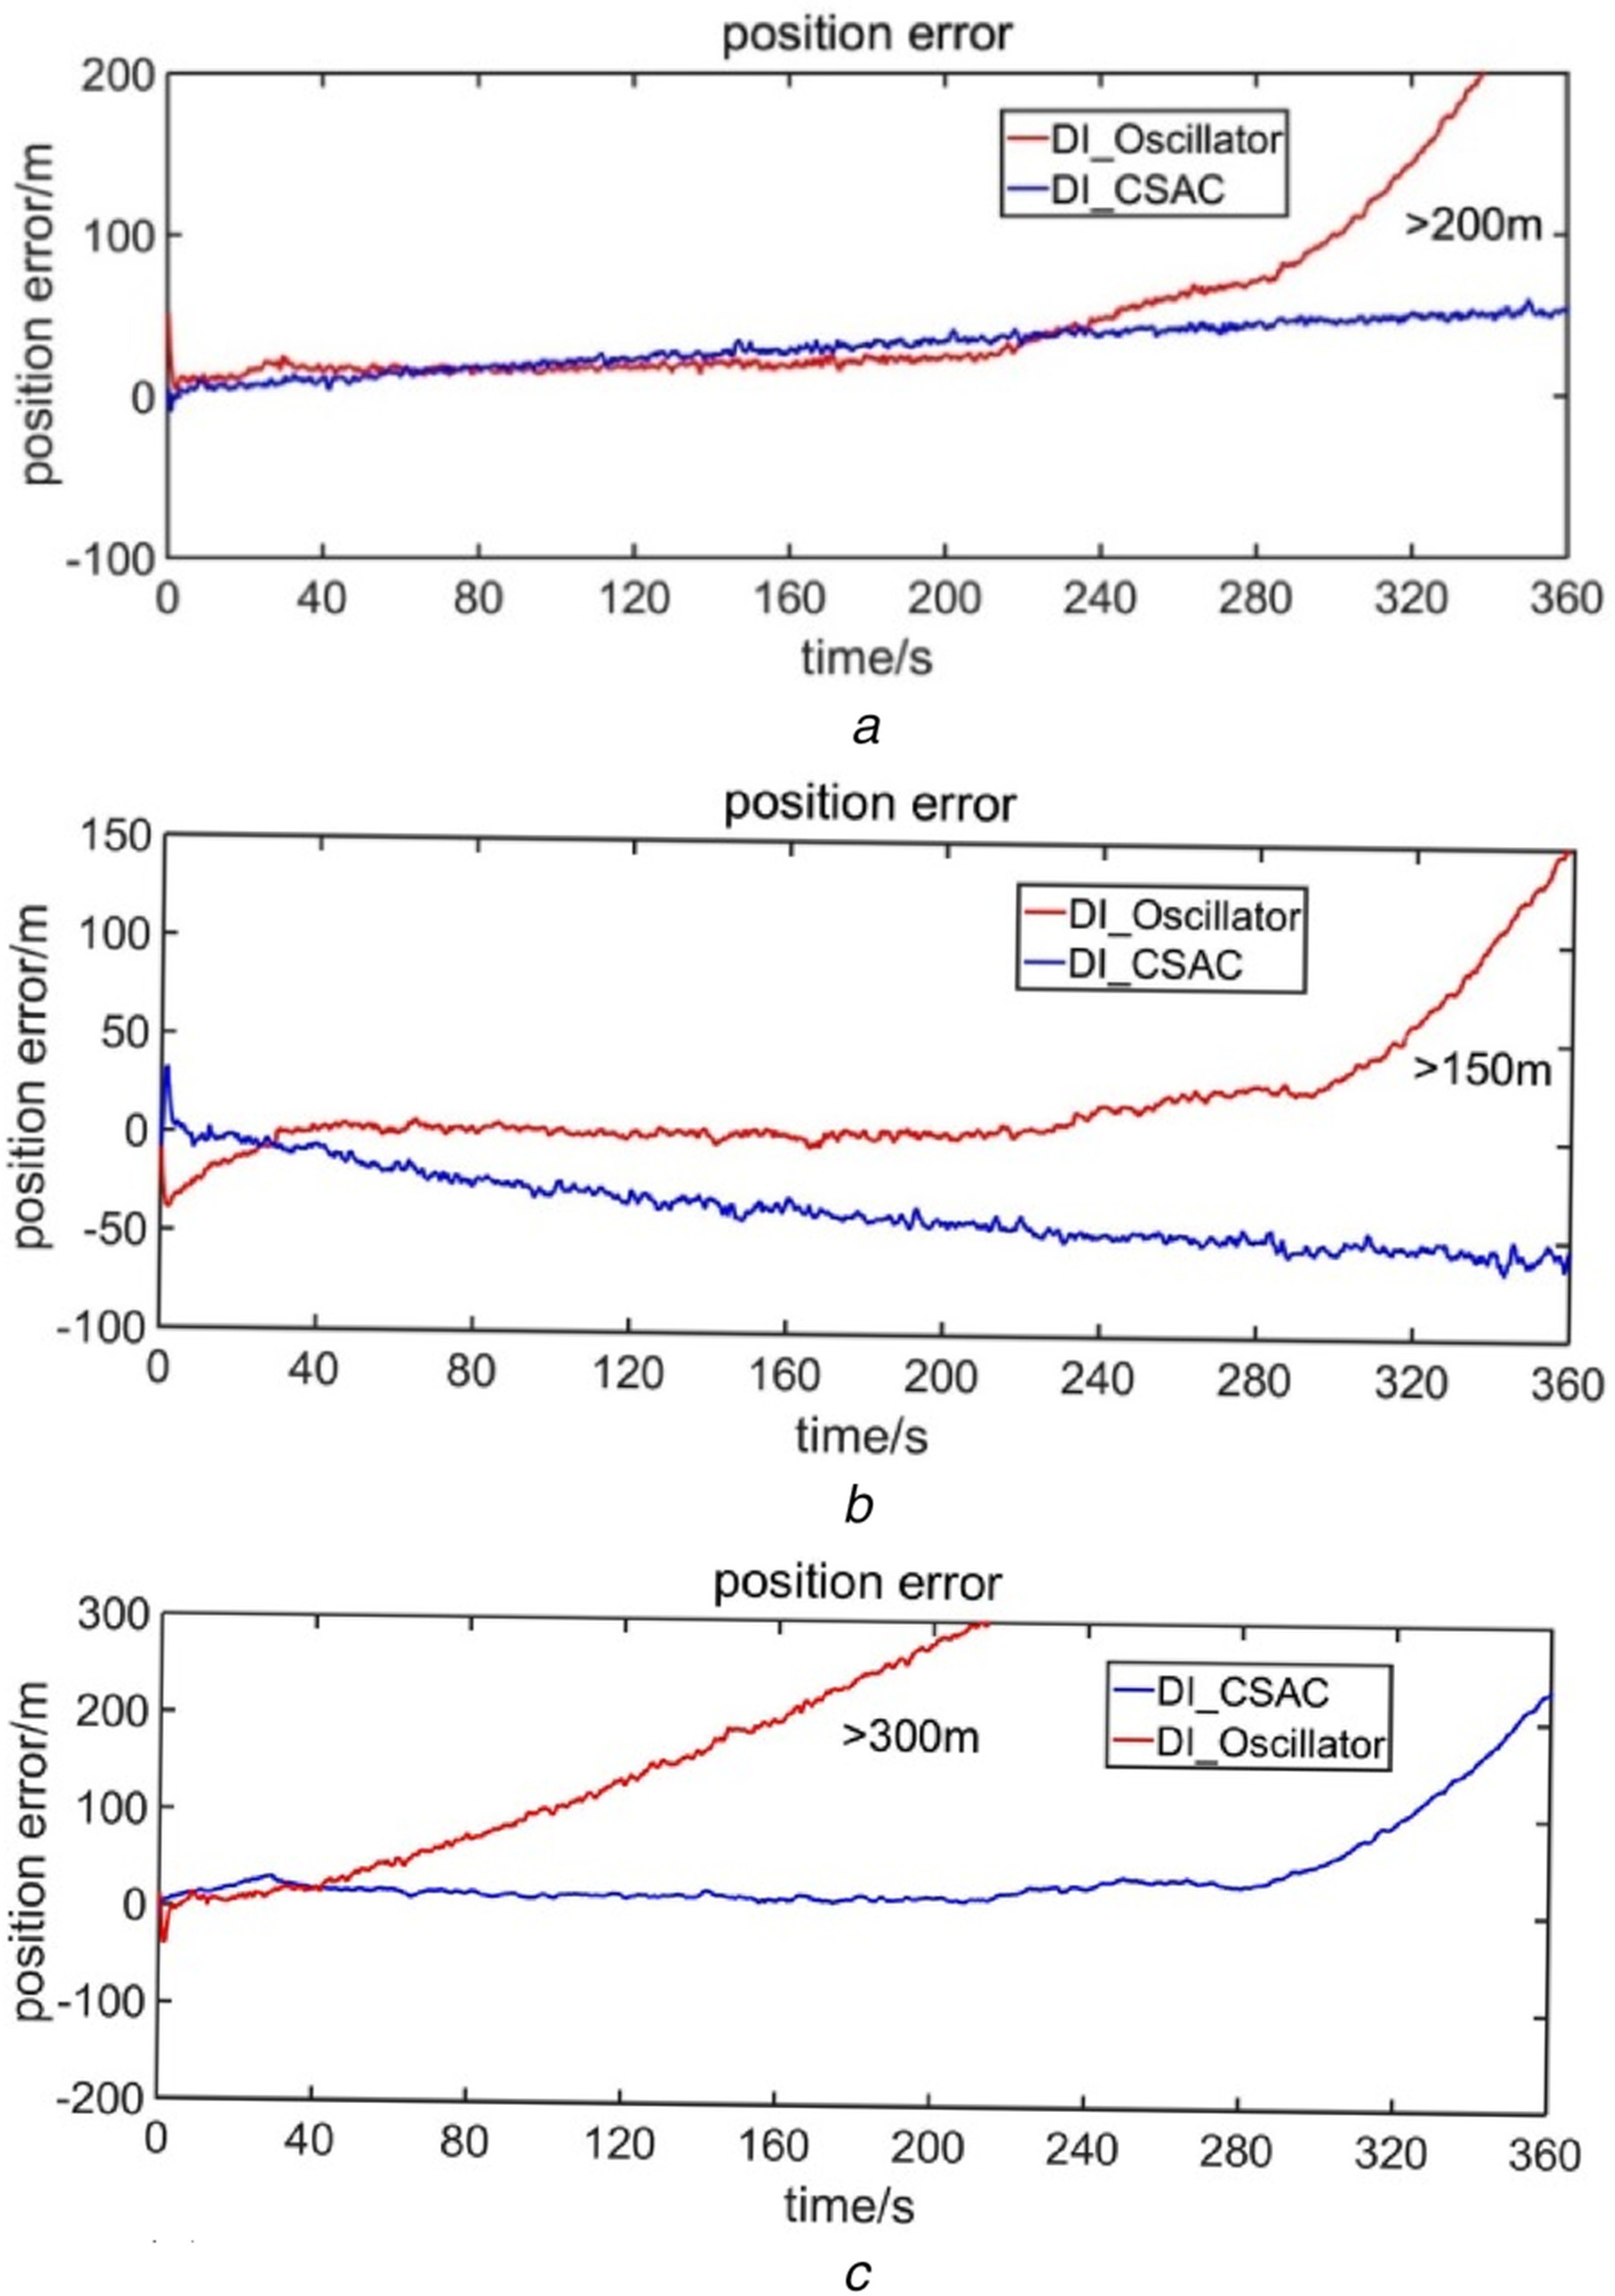
\includegraphics[width=\textwidth]{img/GNSS-errors.jpg}
                \caption{
                    \textcolor[HTML]{3E4091}{TCXO},
                    \textcolor[HTML]{B04A47}{CSAC}
                }
            \end{figure}

        \end{column}

    \end{columns}

\end{frame}


\section{Ocean Bottom Seismic (OBS)}

\begin{frame}{Seismic Methods \& Oil Exploration}

    Seismic or acoustic methods measure the travel times of the reflected or refracted waves detected by a series of geophones and are able to estimate the location and depth of the targets.

    \vspace{10pt}

    \begin{columns}[c, onlytextwidth]

        \begin{column}{0.45\textwidth}

            \begin{figure}
                \centering
                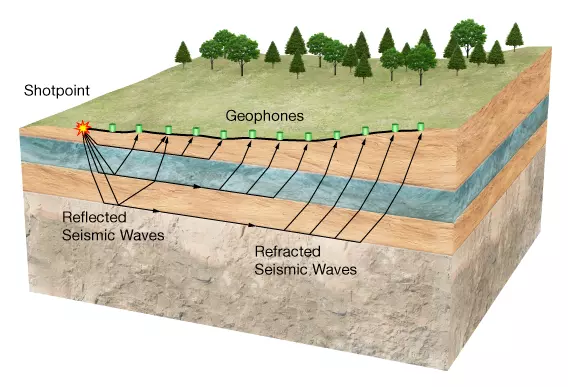
\includegraphics[width=\textwidth]{img/OBS-seimic.png}
                \caption{Seismic method applied from Earth's surface.}
            \end{figure}

        \end{column}

        \hfill

        \begin{column}{0.5\textwidth}

            A \textbf{precise timestamp is required} to measure the travel time of the waves.

            \vspace{10pt}

            Seismic methods are used for oil exploration since they can estimate the location and depth of the oil reservoirs.

        \end{column}

    \end{columns}

\end{frame}



\begin{frame}{Role of CSAC}

    Small short \& medium drifts $\rightarrow$ no GNSS required for nodes synchronization.

    Low battery consumption $\rightarrow$ long-lasting measurements campaigns (weeks or months).

    \begin{figure}
        \centering
        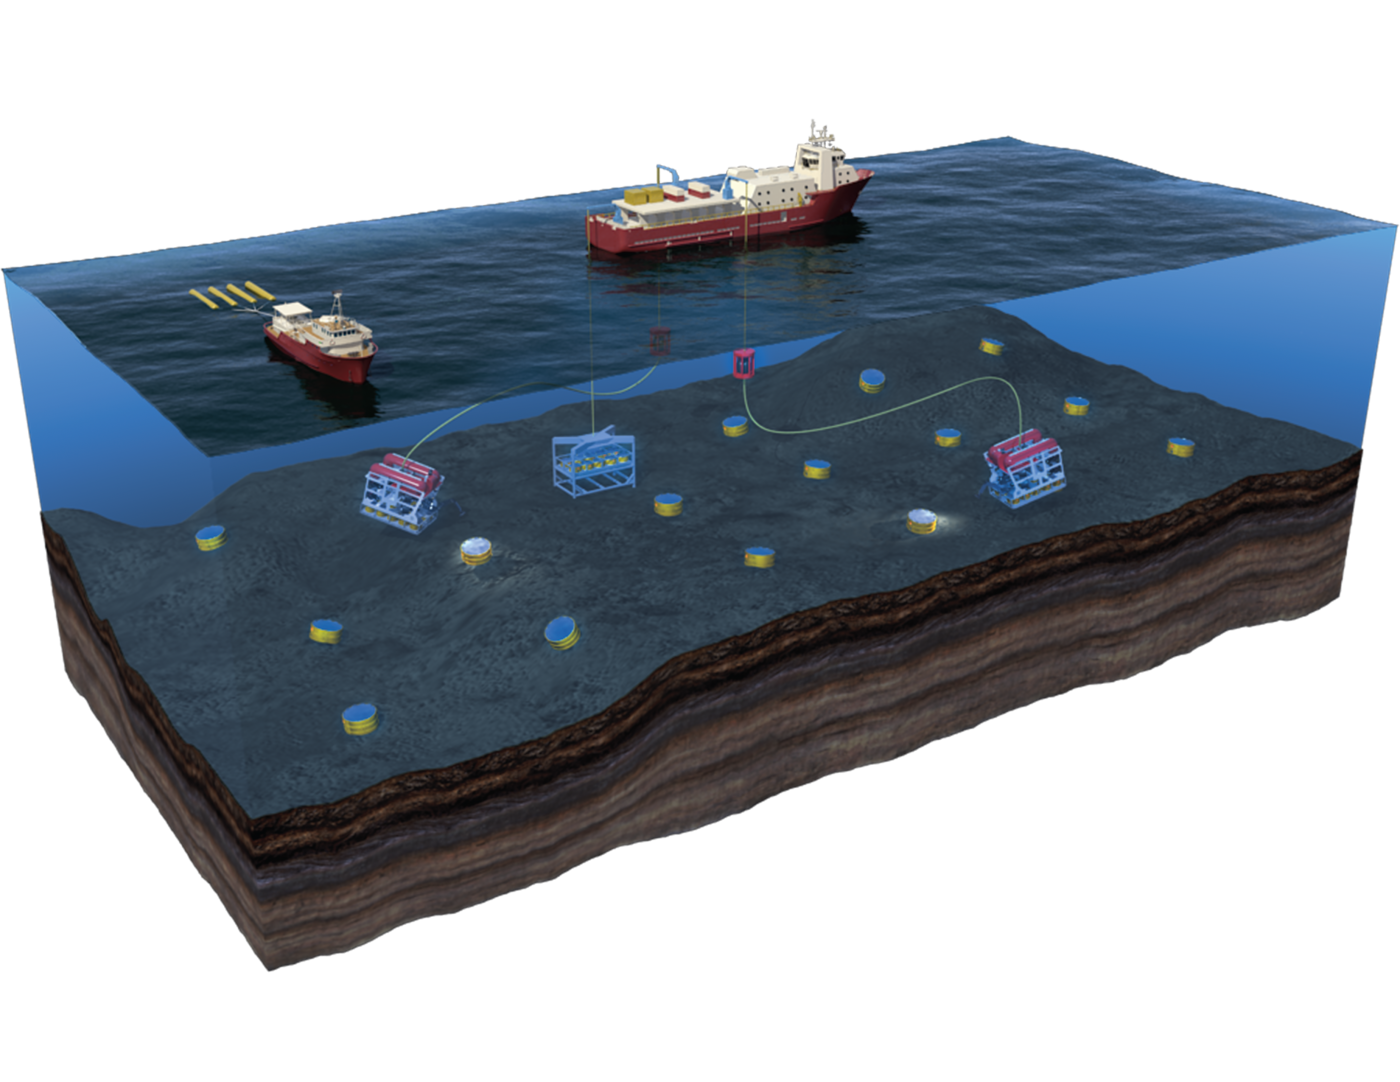
\includegraphics[width=0.5\textwidth]{img/OBS.png}
        \caption{Thanks to CSAC, mapping is now done by placing the geophones on the ocean floor and not on the surface, obtaining more accurate results.}
    \end{figure}

\end{frame}
\section{Military field}

% Example of applications in the military field
% - Anti jamming and spoofing
% - UAVs
% - Missiles
% - Communication systems

\begin{frame}{IED (Improvised Explosive Devices) Jammers}

    \begin{columns}[c, onlytextwidth]

        \begin{column}{0.5\textwidth}

            IED Jammers are devices that prevent the detonation of IEDs by blocking the radio signals used to trigger them.

            \vspace{10pt}

            A single jammer can cover a limited area, so multiple jammers are used to cover a larger area.
            In order to work together, \textbf{the network must be tightly synchronized}.

        \end{column}

        \hfill

        \begin{column}{0.45\textwidth}

            \begin{figure}
                \centering
                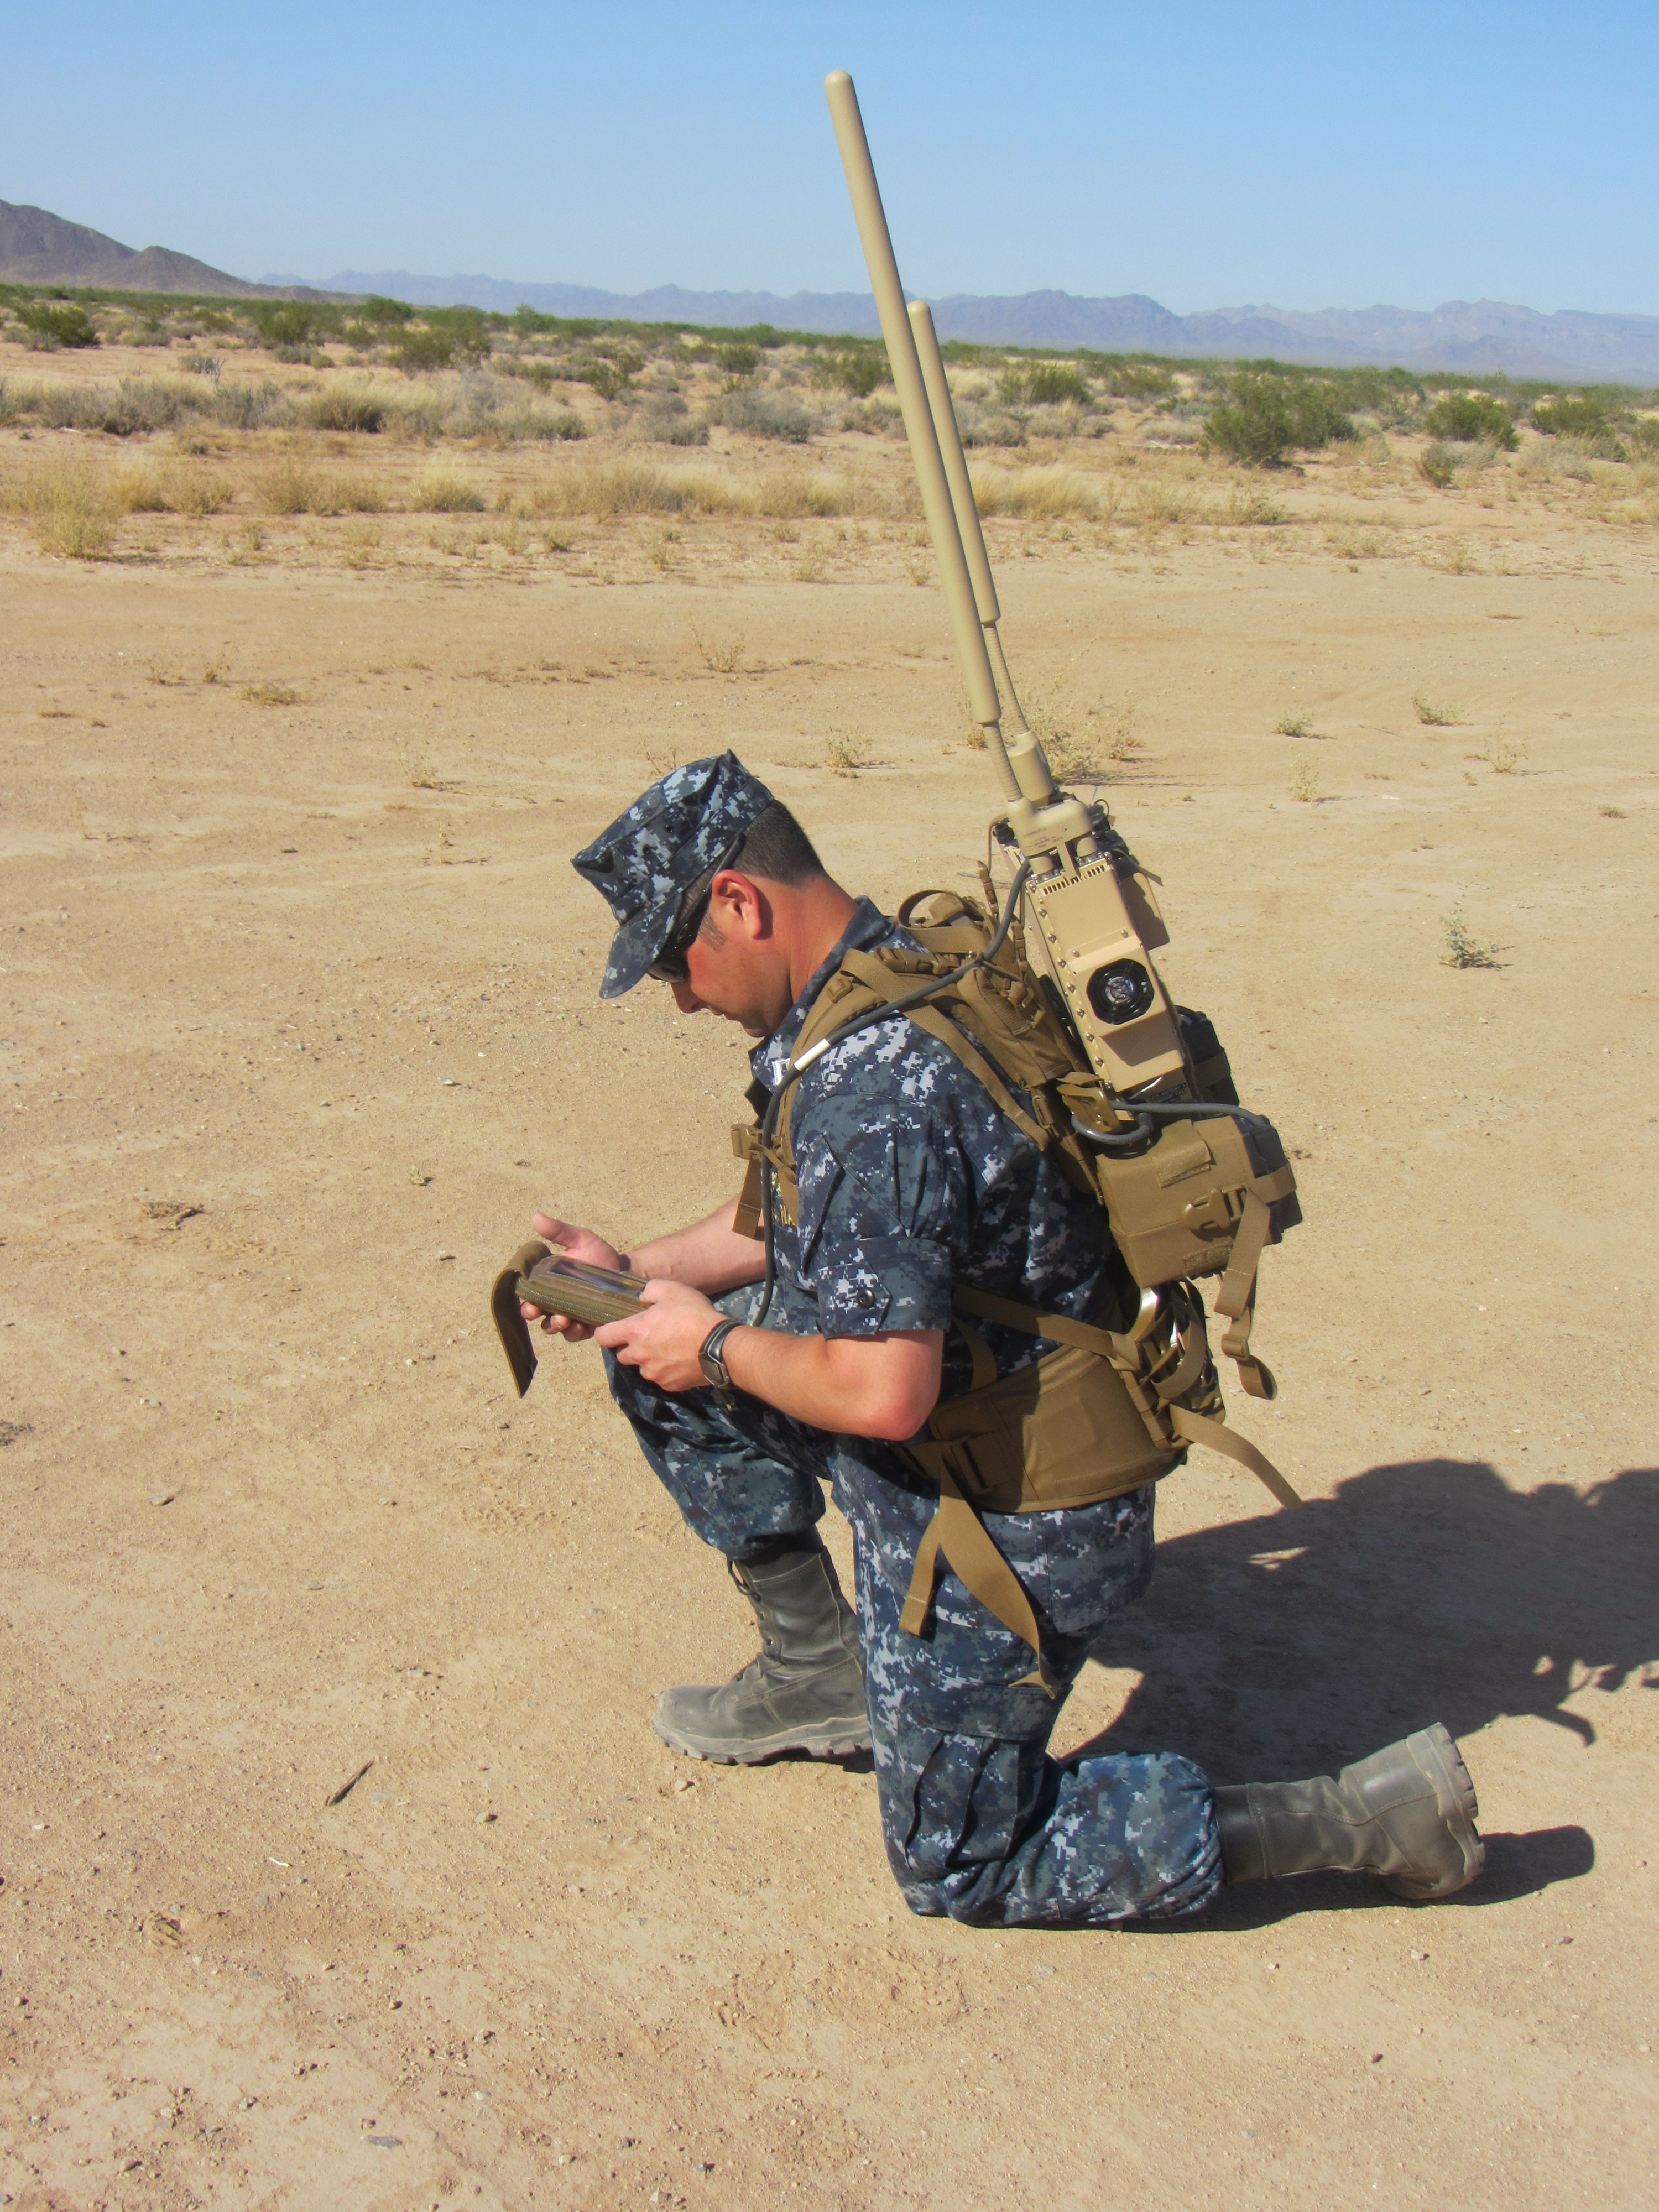
\includegraphics[width=\textwidth]{img/IED-jammers.jpg}
                % \caption{IED Jammers}
            \end{figure}

        \end{column}

    \end{columns}

\end{frame}



\begin{frame}{SAASM (Selective Availability Anti-Spoofing Module)}

    \begin{columns}[c, onlytextwidth]

        \begin{column}{0.35\textwidth}

            \begin{figure}
                \centering
                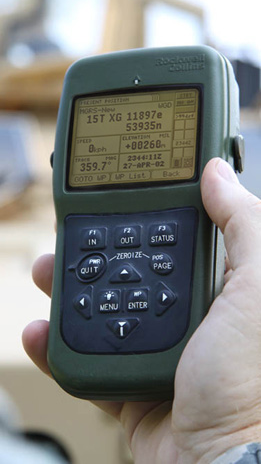
\includegraphics[width=\textwidth]{img/SAASM.png}
                % \caption{IED Jammers}
            \end{figure}

        \end{column}

        \hfill

        \begin{column}{0.6\textwidth}

            SAASM is a module that provides decryption and encryption capabilities to GPS receivers.

            \vspace{10pt}

            The use of a CSAC reduce the time needed to acquire the signal and allows the \textbf{use of longer GPS codes (encrypted P(Y) code)} that are less susceptible to jamming and spoofing.

        \end{column}

    \end{columns}

\end{frame}
\section{Conclusion}

\begin{frame}{Applications of CSACs}

    CSACs find applications in sectors that require \textbf{high precision timing} sources, \textbf{network synchronization} without GNSS, \textbf{low power} consumption and \textbf{portable devices}.

    \vspace{10pt}

    The relative high cost of CSACs ($500\$$ - $5000\$$) is still a barrier to their widespread adoption in large-scale or consumer products.

\end{frame}

\appendix

\begin{frame}[standout]
    Extra slides
\end{frame}



\begin{frame}{5G networks}

    5G networks require highly accurate timing sources for synchronization (max shift in the order of $100 ns/day$).

    In case of failure of the primary source, CSAC holdover capabilities can be used to maintain synchronization at base stations.

    \begin{figure}
        \centering
        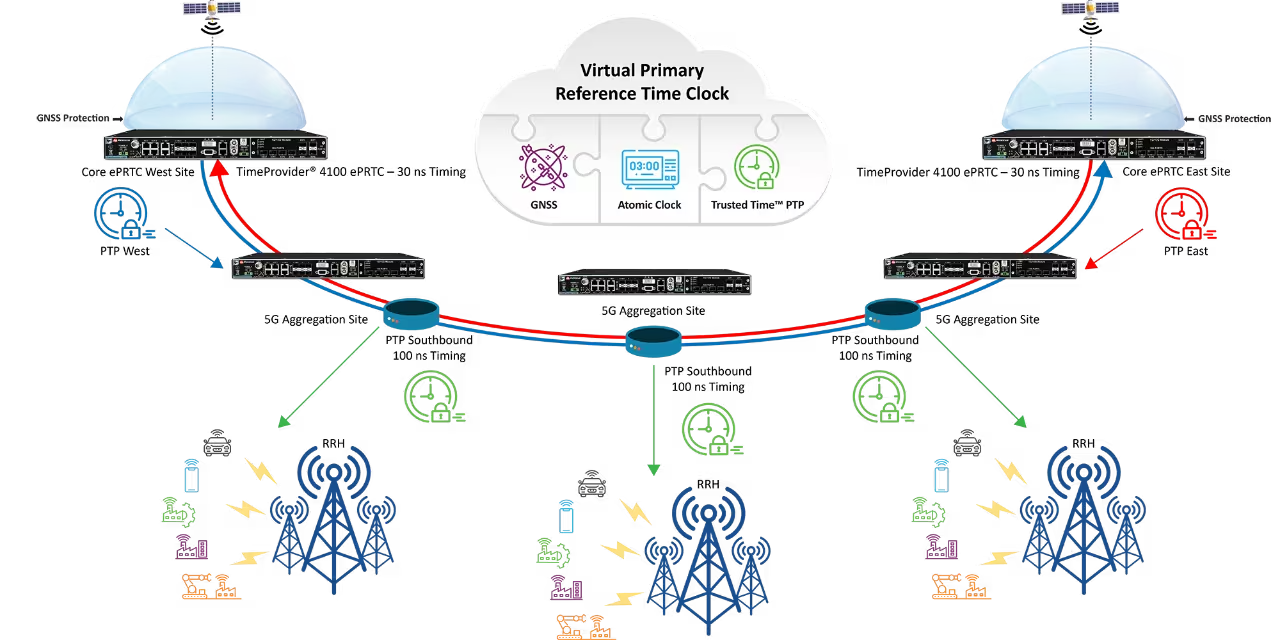
\includegraphics[width=0.8\textwidth]{img/5G.png}
    \end{figure}

\end{frame}



\begin{frame}{Space experiments}

    Space versions of CSACs are being developed for scientific missions and data collection.

    SPATIUM (Space Precision Atomic-clock Timing Utility Mission) is a mission with the objective to model the ionosphere TEC (Total Electron Content) based on multipoint measurements formed by a constellation of small satellites.

    \begin{figure}
        \centering
        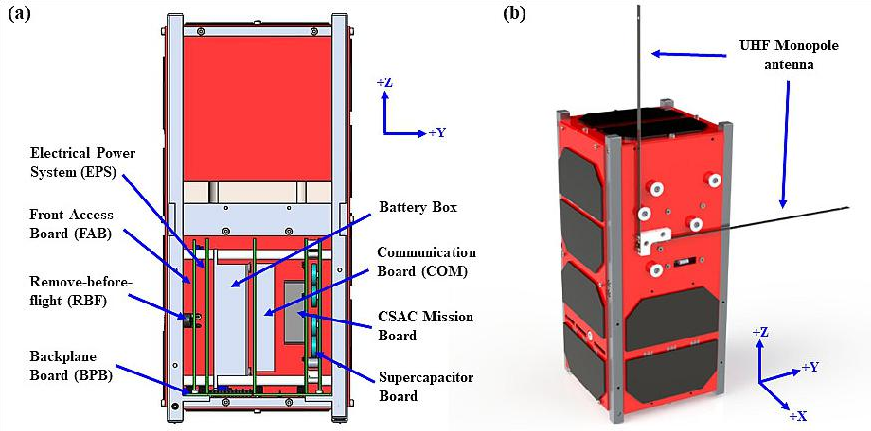
\includegraphics[width=0.8\textwidth]{img/SPATIUM.png}
    \end{figure}

\end{frame}

\begin{frame}[allowframebreaks]{References}
    \nocite{*}
    \bibliography{references}
\end{frame}

\begin{frame}[standout]
    Questions?
\end{frame}

\begin{frame}[standout]
    Thank you!
\end{frame}

\end{document}